\documentclass[crop,tikz]{standalone}

\tikzset{>=latex}
\usetikzlibrary{decorations.markings}
\colorlet{green}{black!40!green}
\definecolor{orange}{RGB}{250,194,25}
\newcommand{\place}{\vec{r}}
\newcommand{\velocity}{\vec{v}}

\begin{document}
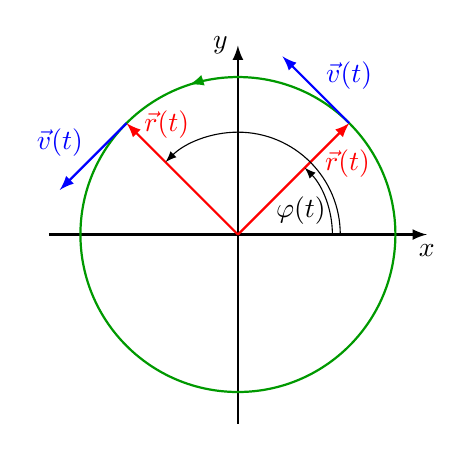
\begin{tikzpicture}[scale=2]
  \draw[->,thick] (-1.2,0) -- (1.2,0) node[below] {$x$};
  \draw[->,thick] (0,-1.2) -- (0,1.2) node[left] {$y$};
  \draw[
    decoration={markings, mark=at position 0.3 with {\arrow{>}}},
    postaction={decorate},
    green,
    thick
  ] (0,0) circle (1);
  % 1
  \draw[->,thick,red] (0,0) -- (45:1);
  \node[red] at (33:0.83) {$\place(t)$};
  \draw[->,thick,blue] (45:1) -- node[right,yshift=0.5em]{$\velocity(t)$} +(135:0.6);
  \draw[->] (0.6,0) arc (0:45:0.6);
  \draw (0.4,0) node[above] {$\varphi(t)$};
  % 2
  \draw[->,thick,red] (0,0) -- (135:1);
  \node[red] at (123:0.83) {$\place(t)$};
  \draw[->,thick,blue] (135:1) -- node[left,yshift=0.5em]{$\velocity(t)$} +(225:0.6);
  \draw[->] (0.65,0) arc (0:135:0.65);
\end{tikzpicture}
\end{document}
